\documentclass[a4paper,fontset = windowsnew]{ctexbook}
\usepackage{xifthen}
\usepackage{calc}
\usepackage{graphicx}
\usepackage{tikz}
\usepackage{cexam}
\usepackage{xcolor}

\begin{document}
\chapter{基本排版程序}

\ExplSyntaxOn

\parindent=0pt

图片与文字的分离程序
%%模块测试

\cexam_sep_pictxt_ii:n 
测试图片
<:
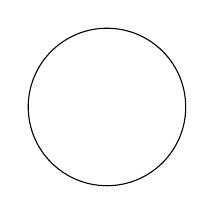
\begin{tikzpicture}
  \draw circle [radius=1];
\end{tikzpicture}
:>
所示的是一个标准的半径为1cm的圆.
\scan_stop:


\par
\cexam_seped_pic:

\par
\cexam_seped_txt:

\end{document}
